\documentclass{article}
\usepackage[T1]{fontenc}
\usepackage[utf8]{inputenc}
\usepackage[english]{babel}
\usepackage{amssymb}
\usepackage{amsthm}
\usepackage{times}
\usepackage{tikz}
\usepackage{color}
\usepackage{pgf}
\usepackage{graphicx}
\usetikzlibrary{calc,through,backgrounds,positioning,fit}
\usetikzlibrary{shapes,arrows,shadows}
\begin{document}
\begin{figure}[!ht]
	\begin{center}
		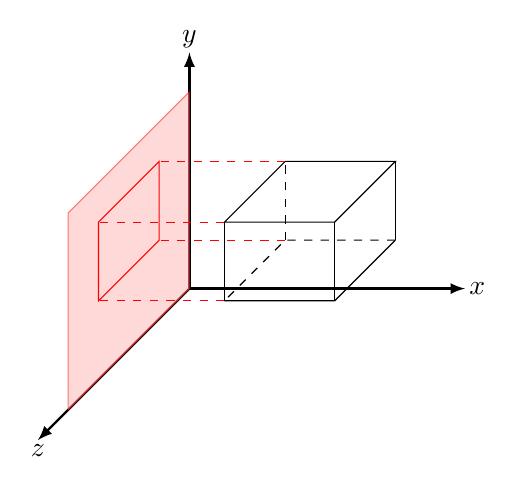
\begin{tikzpicture}[scale=1, inner sep=0.4mm]
		\draw [- latex,thick] (0,0,0) -- (3.5,0,0) node [right] {$x$};
		\draw [- latex,thick] (0,0,0) -- (0,3,0) node [above] {$y$};
		\draw [- latex,thick] (0,0,0) -- (0,0,5) node [below] {$z$};
		
		\filldraw [draw=red,fill=red!30!white,opacity=0.5] (0,0,4) -- (0,0,0) -- (0,2.5,0) -- (0,2.5,4) -- cycle;
		
		\draw  (1.6,2, 1) -- (1.6,2,3) -- (3,2,3) -- (3, 2, 1) --cycle;		
		\draw[dashed] (3, 1, 1)-- (1.6, 1, 1) -- (1.6, 1, 3);
		\draw (1.6, 1, 3) -- (3, 1, 3) -- (3, 1, 1);
		\draw (3, 2, 3)--(3, 1, 3) (1.6, 2, 3)--(1.6, 1, 3) (3, 2, 1)--(3, 1, 1) ;
		\draw [dashed] (1.6, 1, 1)--(1.6, 2, 1);		 

		\draw[draw= red,dashed] (1.6, 1, 1) -- (0, 1, 1);
		\draw[draw= red,dashed] (1.6, 2, 3) -- (0, 2, 3);
		\draw[draw= red,dashed] (1.6, 1, 3) -- (0, 1, 3);
		\draw[draw= red,dashed] (1.6, 2, 1) -- (0, 2, 1);
		
		\draw[draw= red]  (0, 1, 1) -- (0, 2, 1)  -- (0,2,3) -- (0, 1, 3) --cycle;		
		

		\end{tikzpicture}
	\end{center}
\end{figure}
\end{document}